\section{计算软件PHONOPY}\label{sec:计算软件PHONOPY}

\sectionAuthor{Isay K.}

在本节,你将要学到:
\begin{Abstract}
    \item 开始安装之前
    \item PHONOPY快速安装
    \item PHONOPY使用方法
\end{Abstract}

\subsection{开始安装之前}\label{subsec:计算软件PHONOPY-开始安装之前}

由于本教程面向的群体是计算小白(包括笔者也是通过本教程记录一下自己掉的坑),所以在开始安装软件之前,我们强烈建议先咨询组内老师或师兄师姐:服务器上是否已经配置了相应的软件?

\begin{extend}
    当然也可以使用 module avail 命令自己检查系统内已安装的软件,如果没有找到的话再咨询更有自主性哦。
    \begin{figure}
        \centering
        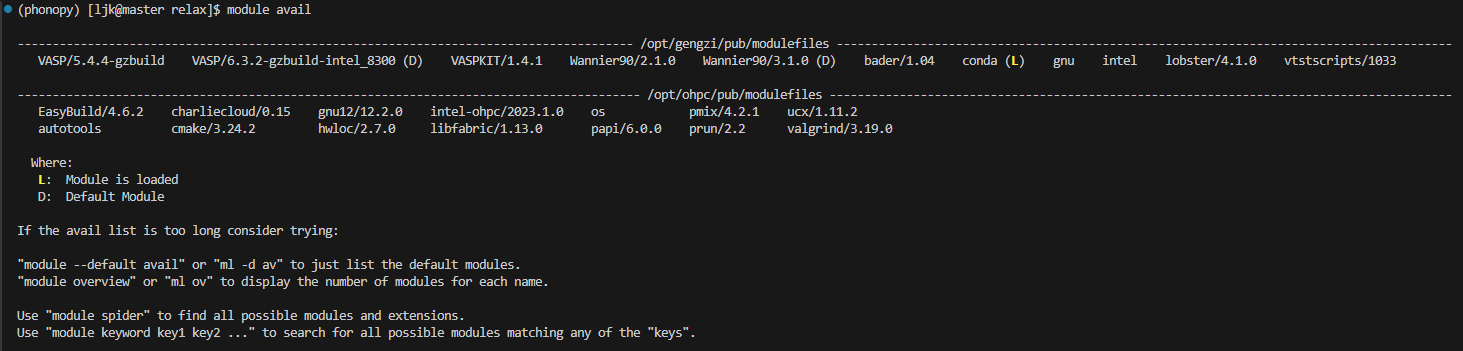
\includegraphics[width=1\linewidth]{module-check.png}
        \caption{检查是否含有所需软件}
        \label{fig:检查软件}
    \end{figure}
\end{extend}

通常情况下,组内服务器的\emph{根目录}下已经配置了相应的软件,这个时候再在自己的\emph{用户目录}下进行配置的话,一方面在使用过程中可能会出现命令的冲突,另一方面也是一种时间、精力和资源的浪费。

如果组内确实并没有安装,或者你是传说中的开山大弟子,又或者是自学,请放心进入\ref{subsec:计算软件PHONOPY-PHONOPY快速安装}小节。

\subsection{PHONOPY快速安装}\label{subsec:计算软件PHONOPY-PHONOPY快速安装}

% 聪明的小朋友从图\ref{fig:检查软件}中其实已经可以看出端倪,图中并没有PHONOPY模块。

% 这是因为使用传统的安装方式较为麻烦,而且PHONOPY新版本需要\emph{python>=3.7.0},需要自行安装python等多个模块。因此我们借助一个神器——Anaconda——进行PHONOPY的安装。

% 写着写着突然想起
% \subsubsection{Anaconda安装}

% Anaconda的官网:
% https://www.continuum.io/downloads/

% 官网需要翻墙,可以使用清华的镜像网站:
% https://mirrors.tuna.tsinghua.edu.cn/anaconda/archive/

% \begin{figure}
%     \centering
%     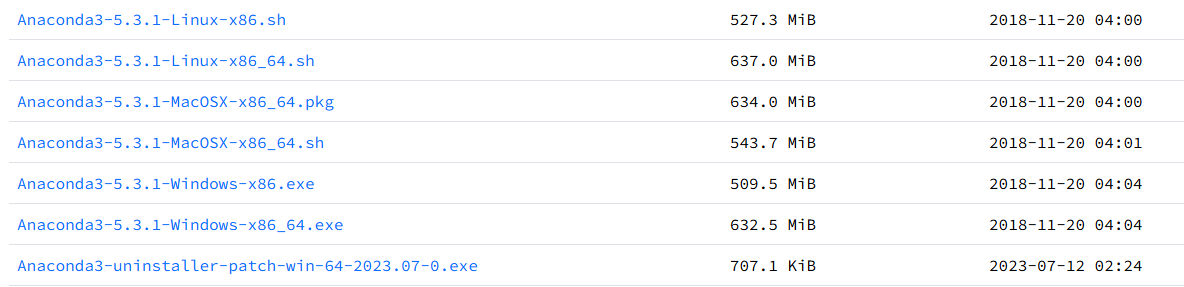
\includegraphics[width=1\linewidth]{mirror.png}
%     \caption{镜像网站}
%     \label{fig:镜像网站}
% \end{figure}

% 图\ref{fig:镜像网站}中,x86是32位的,x86\_64是64位的,根据服务器的系统型号下载即可。

% 将下载好的.sh文件放在服务器的根目录下,进入该目录

参考:
https://blog.csdn.net/qq\_41866202/article/details/124407208?spm=1001.2101.3001.6661.1\&utm\_medium=distribute.pc\_relevant\_t0.none-task-blog-2\%7Edefault\%7EBlogCommendFromBaidu\%7ECtr-1-124407208-blog-139391379.235\%5Ev43\%5Epc\_blog\_bottom\_relevance\_base9\&depth\_1-utm\_source=distribute.pc\_relevant\_t0.none-task-blog-2\%7Edefault\%7EBlogCommendFromBaidu\%7ECtr-1-124407208-blog-139391379.235\%5Ev43\%5Epc\_blog\_bottom\_relevance\_base9\&utm\_relevant\_index=1

\subsection{PHONOPY使用方法}\label{subsec:计算软件PHONOPY-PHONOPY使用方法}

\subsubsection{加载PHONOPY环境}
\begin{enumerate}
    \item 加载Anaconda应用:\code{module load conda}
    \item 激活PHONOPY环境:\code{conda activate PHONOPY}
\end{enumerate}

\subsubsection{命令详解}

进入下面的官网之后点击Command options即可看到所有功能。

https://phonopy.github.io/phonopy/index.html 

\begin{attention}
 在进行扩胞时的标准是:扩胞后的原子达到80\ttilde100个,每个晶轴方向大于10,不然得到的声子谱中很容易出现虚频。
\end{attention}